\documentclass{article}
\usepackage[russian]{babel}
\usepackage[utf8]{inputenc}
\usepackage{amsthm}
\usepackage{amsmath}
\usepackage{amsfonts}
\usepackage{mathtools}
\usepackage{graphicx}

\newtheorem{lemma}{Лемма}
\newtheorem{definition}{Определение}
\newtheorem{theorem}{Теорема}

\begin{document}
	\begin{definition}
		Циклической перестановкой из $k$ элементов с шагом $s$ будем называть такую циклическую перестановку, в которой элемент с номером $i$ переходит в элемент с номером $i+s \hspace{5pt} (\mod k)$. 
	\end{definition}

	Далее будем считать, что элементы перестановки длины $k$ - это числа от $0$ до $k-1$.
	
	\begin{lemma}
		Пары перестановок вида $xy$ и $yx$ пробегают в том числе всевозможные пары циклических перестановок длины $k$ с произвольным шагом. 
	\end{lemma}

	\begin{proof}
		Зафиксируем произвольные $s$ и $t$ из \{$0$, .., $k-1$\} и докажем, что найдутся такие перестановки $x$ и $y$ из $k$ элементов, что $xy$ будет циклической перестановкой с шагом $s$, а $yx$ - циклической перестановкой с шагом $t$.
		
		
		Пусть элемент $i$ переходит под действием перестановки $x$ в элемент $x_i$. Потребуем, чтобы $x_i$ под действием перестановки $y$ перешел в $i + s$ ($\mod k$). $i + s$ в свою очередь под действием $x$ переходит в $x_{i+s}$, потребуем, чтобы $x_{i+s}$ = $x_i + t$ ($\mod k$).
		
		\begin{equation}
			i \xrightarrow{x} x_i \xrightarrow{y} i+s \xrightarrow{x} x_{i+s} = x_i + t
		\end{equation}
		
		Поскольку $\{x_i\}$ = $\{x_{i+s}\}$ - множество всех остатков от деления на $k$, то $\{x_i + t\}$ ($\mod k$) - также множество всех остатков от деления на $k$. Все $x_i$ и $x_i + t$ различны. 
		Получим систему из $k$ равенств вида $x_{i+s}$ = $x_i + t$ ($\mod k$), $i \in \{0, ..., k-1\}$, где $x_i, x_{i+s} \in \{0, ..., k-1\}$ и каждое такое число встречается по разу в левой и в правой части. Такая система имеет $k$ решений.
		
	\end{proof}
	
	\begin{lemma}
		Пусть $(xy)^a(yx)^b(xy)^c$ = $(yx)^c(xy)^b(yx)^a$ - тождество в $S_k$. Тогда $a - b + c \equiv 0 \hspace{5pt} (\mod k)$.
	\end{lemma}
	\begin{proof}
		Зафиксируем произвольные $s$,  $t$ $\in \{0, ..., k-1\}$. По Лемме 1 существуют такие перестановки $x$ и $y$, что $xy$ и $yx$ - это циклические перестановки с шагами $s$ и $t$ соответственно. Рассмотрим перестановочный автомат, в котором переход по символам осуществляется соответствующими перестановками $x$ и $y$. Тогда, чтобы $(xy)^a(yx)^b(xy)^c$ = $(yx)^c(xy)^b(yx)^a$ было тождеством для такого автомата, требуется, чтобы автомат закончил читать обе части равенства в одном состоянии, то есть	
		\begin{equation}
			as + bt + cs \equiv ct + bs + at \hspace{5pt} (\mod k)
		\end{equation}
		что эквивалентно 
		\begin{equation}
		(a - b + c)(s - t) \equiv 0 \hspace{5pt} (\mod k)
		\end{equation}
		Поскольку $s$ и $t$ принимают произвольные значения $\{0, ..., k-1\}$, их разность по модулю $k$ также принимает различные значения из $\{0, ..., k-1\}$. Найдутся такие $s$ и $t$, $s-t$ будет взаимно просто с $k$. Откуда $a - b + c$ должно делиться на $k$.
	\end{proof}

	\begin{lemma}
		Существуют такие перестановки $x$ и $y$, что $xy$ - циклическая перестановка с шагом 1, а $yx$ - циклическая перестановка с шагом 1, в которой поменяли местами элементы $a$ и $b$.
	\end{lemma}
	\begin{proof}
		Без ограничения общности $a < b$.
		Требуется, чтобы $xy$ = (0, 1, 2, ..., $k-1$), а $yx$ = (0, 1, ..., $a-1$, $b$, $a+1$, ..., $b-1$, $a$, $b+1$, ..., $k-1$).
		
		Пусть $x$ переводит $a-1$ в $b$, $b-1$ в $a$, а любой другой элемент в следующий, то есть
		$$
		x = 
		\begin{pmatrix}
			0&...&a-2&a-1&a&...&b-2&b-1&b&...\\
			1&...&a-1&b&a+1&...&b-1&a&b+1&...
		\end{pmatrix}
		$$
		а $y$ переводит $a$ в $b$ и наоборот, а остальные элементы оставляет на месте:
		
		$$
		y = 
		\begin{pmatrix}
			0&...&a-1&a&a+1&...&b-1&b&b+1&...\\
			0&...&a-1&b&a+1&...&b-1&a&b+1&...
		\end{pmatrix}
		$$
		Откуда получим 
		$$
		xy = 
		\begin{pmatrix}
			0&...&a-2&a-1&a&...&b-2&b-1&b&...\\
			1&...&a-1&a&a+1&...&b-1&b&b+1&...
		\end{pmatrix}
		$$
		$$
		yx = 
		\begin{pmatrix}
			0&...&a-2&a-1&a&...&b-2&b-1&b&...\\
			1&...&a-1&b&b+1&...&b-1&a&a+1&...
		\end{pmatrix}
		$$
		Что и требовалось найти.
	\end{proof}

	\begin{theorem}
		 Пусть $(xy)^a(yx)^b(xy)^c$ = $(yx)^c(xy)^b(yx)^a$ - тождество в $S_k$. Тогда выполняется хотя бы одно из следующих правил:
		 \begin{equation*}
		 k|a \hspace{10pt} \text{и} \hspace{10pt} k|(b-c)
		 \end{equation*}
		 \begin{equation*}
		 k|c \hspace{10pt} \text{и} \hspace{10pt} k|(b-a)
		 \end{equation*}
		 \begin{equation*}
		 k|b \hspace{10pt} \text{и} \hspace{10pt} k|(a+c)
		 \end{equation*}
	\end{theorem}
	\begin{proof}
		От противного. Допустим, ни одно из перечисленных правил не выполняется, то есть ни одно из чисел $a$, $b$, $c$ не делится на $k$. Тогда с учетом Леммы 2 на $k$ не делятся и числа $b-a$, $b-c$, $a+c$. Тогда найдутся автоматы, различающие строки справа и слева от знака равенства. Рассмотрим несколько случаев.
		
		\begin{enumerate}
			\item $a+b \ne 0 \mod k$
			
			Рассмотрим перестановочный автомат такой, что $xy$ действует на него как циклическая перестановка из $k$ элементов с шагом 1, а $yx$ - как циклическая перестановка из $k$ элементов с шагом 1, в которой поменяли местами элементы $a+b$ и $a+c$ (см. Рис. \ref{cycle_a+b_a+c}). $a+b$ и $a+c$ не равны 0 по модулю $k$, $a+b \ne a+c$, так как $b-c$ не делится на $k$. (Существование такого автомата доказывает Лемма 3). Начальное состояние 0.
			
			\begin{figure}
				\centering{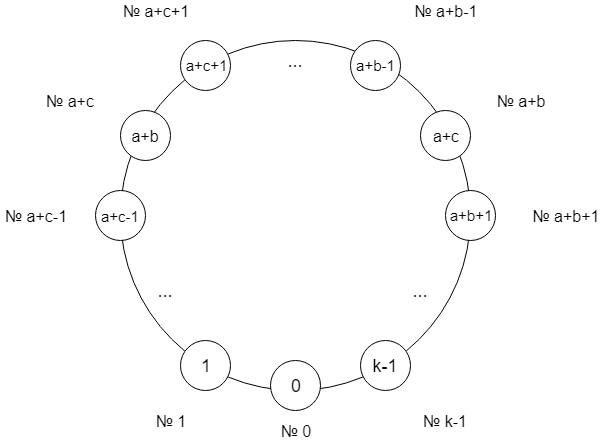
\includegraphics[scale=0.5]{images/cycle_a+b_a+c}}
				\caption{Перестановка $yx$}
				\label{cycle_a+b_a+c}
			\end{figure}
		
			Покажем, что такой автомат различит слова $(xy)^a(yx)^b(xy)^c$ и $(yx)^c(xy)^b(yx)^a$.\\
			
			Автомат закончит читать слово $(xy)^a(yx)^b(xy)^c$ в состоянии $a+2c$ (см. Рис \ref{process1_cycle_a+b_a+c}).
			Корректность переходов:
			\begin{itemize}
				\item $a \ne a+b$, так как $b \not \equiv 0 \mod k$
				\item $a \ne a+c$, так как $c \not \equiv 0 \mod k$
				\item $a+2c$
			\end{itemize}
			
			\begin{figure}
				\centering{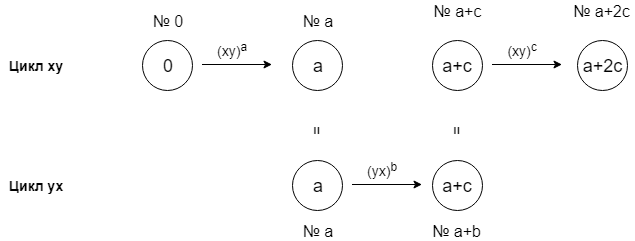
\includegraphics[scale=0.5]{images/process1_a+b_a+c}}
				\caption{Чтение автоматом слова $(xy)^a(yx)^b(xy)^c$}
				\label{process1_cycle_a+b_a+c}
			\end{figure}
			
		\end{enumerate}
	\end{proof}
\end{document}